\documentclass{article}

\usepackage{fullpage}
\usepackage[utf8]{inputenc} % allow utf-8 input
\usepackage[T1]{fontenc}    % use 8-bit T1 fonts
\usepackage{hyperref}       % hyperlinks
\usepackage{url}            % simple URL typesetting
\usepackage{booktabs}       % professional-quality tables
\usepackage{amsmath}
\usepackage{amssymb}
\usepackage{amsfonts}       % blackboard math symbols
\usepackage{mathtools}
\usepackage{nicefrac}       % compact symbols for 1/2, etc.
\usepackage{microtype}      % microtypography
\usepackage{algorithm}
\usepackage{algpseudocode}
\usepackage{graphicx}
\usepackage{float}
\usepackage{caption}
\usepackage{outlines}
\usepackage{tikz}
\usepackage{dsfont}
\usepackage{empheq}
\usepackage{xfrac}
\usepackage{enumitem}
\usepackage{amsthm}
%\usepackage{geometry}
%\geometry{margin=1.5in}

\theoremstyle{definition}

\newtheorem{thm}{Theorem}
\newtheorem{lemma}[thm]{Lemma}
\newtheorem{claim}[thm]{Claim}
\newtheorem{defn}[thm]{Definition}

\newcommand{\nth}{^{\text{th}}}
\newcommand{\len}{\text{len}}
\newcommand{\indicator}{\mathds{1}}
\newcommand{\hackystatei}[1]{\State \parbox[t]{\dimexpr\linewidth-\algorithmicindent}{#1\strut}}
\newcommand{\hackystateii}[1]{\State \parbox[t]{\dimexpr\linewidth-\algorithmicindent-\algorithmicindent}{#1\strut}}
\newcommand{\argmax}{\mathop{\mathrm{argmax}}}
\newcommand{\argmin}{\mathop{\mathrm{argmin}}}

\newcommand{\Dirichlet}{\text{Dirichlet}}
\newcommand{\Categorical}{\text{Categorical}}
\newcommand{\Exit}{\textsc{Exit}}

\newcommand{\leaves}{\text{leaves}}
\newcommand{\nonTerm}{\text{nonTerm}}
\newcommand{\domain}{\text{domain}}

\newcommand{\tallbracketl}[2]{\left #1 \rule{0ex}{#2} \right.}
\newcommand{\tallbracketr}[2]{\left. \rule{0ex}{#2} \right #1}

\newcommand{\deltaMin}{\delta_{\text{min}}}
\newcommand{\alphaMax}{\alpha_{\text{max}}}
\newcommand{\LCA}{\text{LCA}}
\newcommand{\RbarEst}{\Rbar^\text{(est)}}
\newcommand{\leaf}{\text{leaf}}

\newcommand{\TODOcite}{[?]}

%\allowdisplaybreaks

\title{Inferring Hierarchies of Topics from Co-occurrence Probabilities}

\author{
  Andrew Leverentz \\
  \texttt{aleveren@eng.ucsd.edu} \\
  Sanjoy Dasgupta \\
  \texttt{dasgupta@eng.ucsd.edu}
}

\date{}

\begin{document}

\maketitle

%%%%%%%%%%%%%%%%%%%%%%%%%%%

\section{Introduction}

Traditional probabilistic topic models, such as Latent Dirichlet Allocation (LDA) \TODOcite{}, treat observed documents as mixtures of latent topics, which are in turn viewed as probability distributions over a vocabulary of words.
In LDA, the topics themselves are assumed to co-occur with each other within documents by drawing topic proportions from a symmetric Dirichlet.
However, one may wish to view topics as being members of a hierarchy, in which topics can have varying levels of specificity or generality, and in which sub-topics are more likely to occur with super-topics (corresponding to ancestors in the hierarchy) than they are to occur with non-ancestors.

Several models exist which generalize the ``flat'' collections of topics produced by LDA into hierarchies.
In one class of models, we specify \emph{a priori} a fixed tree (or, more generally, a fixed DAG), and we infer a topic to associate with each leaf node.
In a second class of models, neither the topics nor the tree structure are fixed prior to inference, and Bayesian non-parametric techniques are used to discover a tree of potentially unbounded size.
Here, we will consider Pachinko Allocation Modeling (PAM) \TODOcite{} as a representative of the first type, and the Nested Hierarchical Dirichlet Process (NHDP) \TODOcite{} as a representative of the second type.
NHDP has the advantage of not requiring knowledge of the true structure of the topic hierarchy prior to inference;
however, because its underlying probabilistic model is significantly more complex than PAM, inference for NHDP is relatively cumbersome.

This paper defines a new method for deriving a hierarchy of topics which attempts to combine the desirable aspects of both of the above classes of models.
Unlike PAM, our model does not require specifying a fixed tree structure \emph{a priori}, but our method is significantly simpler and faster than the inference algorithms currently available for NHDP.
Moreover, we offer proof that, under certain assumptions on the data-generating process, our method is capable of exactly recovering the ``true'' tree of topics (with high probability given sufficient data).

\section{A Review of LDA, PAM, and NHDP Topic Models}

\subsection{Latent Dirichlet Allocation (LDA)}

TODO: short introduction to LDA model's assumptions and structure (maybe also mention CTM: correlated topic model?)

\subsection{Inference Algorithms for LDA}

TODO: discussion of Gibbs sampling, variational inference

\subsection{Pachinko Allocation Modeling (PAM)}

Pachinko Allocation Modeling (PAM) provides one way to generalize LDA and incorporate nested hierarchies of topics.
The fully general formulation of PAM consists of a directed acyclic graph $G$ containing a single source node (the ``root''), a Dirichlet distribution over the vocabulary (the ``vocabulary Dirichlet''), and a collection of Dirichlet distributions (one for each internal node), where each node's Dirichlet parameter has a number of components equal to the number of outgoing edges at that node.
The generative model for the general formulation of PAM functions as follows: First, we use the vocabulary Dirichlet to draw one distribution over the vocabulary for each terminal node in the DAG.
This defines a mapping from terminal nodes to topics.
Next, for each document in the corpus, we use the per-node Dirichlet distributions to draw a probability distribution over outgoing edges corresponding to each internal node.
For each word-slot in each document, we select a terminal node by stochastically building a path from the root to a terminal node, using the current document's outgoing-edge probabilities.
Then, we draw a word from the vocabulary using the topic (i.e., the distribution over the vocabulary) corresponding to the selected terminal node.
Similar to LDA, we can infer this model's parameters using standard latent-variable approaches such as Gibbs sampling or variational inference.

The paper which introduced PAM (\TODOcite{}) focused primarily on one particular class of PAM models, which we will refer to as ``4-layer PAM.''
In this model, the DAG actually contains three layers of nodes, since the authors of the original PAM paper consider the topics themselves---which are distributions over the vocabulary---to be the fourth layer.
The first layer (containing only the root node) is fully connected to the second layer, and the second layer is fully connected to the third layer.
Thus, the structure of the DAG is fully specified by indicating the size of the second and third layers of the graph.
We mention this particular variant because the topic-modeling literature occasionally uses ``PAM'' to refer specifically to the 4-layer PAM.
However, in this paper, we will use ``PAM'' to refer to the generic PAM model defined above, rather than the more specialized 4-layer model.

Next, we will consider another special case of PAM which we will refer to as ``TreePAM.''
TreePAM is essentially the same as the generic version of PAM, except the DAG must be a tree (i.e., there is only one path from the root to each node).
Without loss of generality, we may further assume that there are no nodes with exactly one incoming edge and exactly one outgoing edge; this is because such nodes may be removed from the model without changing the generative distribution it defines.
This paper will focus primarily on TreePAM, as it naturally reflects the notion of nested hierarchies of topics.

\subsection{Nested Hierarchical Dirichlet Process (NHDP)}

TODO: short introduction to NHDP model, mention variational inference, and ability to view it as special (infinite) case of TreePAM

\section{A Motivating Observation}

The ``anchor words'' algorithm \TODOcite{} is a non-probabilistic alternative to traditional LDA inference algorithms such as Gibbs sampling or variational inference.
Its main appeals are (1) its relatively fast runtime, (2) provable guarantees on its ability to recover the topics with which a given dataset was generated, and (3) its ability to handle non-trivial co-occurrence patterns.
The anchor-words algorithm produces a matrix $A$ representing the topics appearing in the corpus (each row of $A$ corresponds to a probability distribution over the vocabulary).
In addition, it produces a matrix $R$ representing the probabilities of pairs of topics co-occurring within a single document.
One of the observations that motivated this paper was that, when a corpus is generated according to a hierarchical topic model such as PAM, the $R$ matrix recovered by the anchor-words algorithm appears to contain significant information about the structure of the underlying hierarchy.
(TODO: include a figure demonstrating the structure that is visible in the $R$ matrix.)
Thus, a natural question to ask is, can we recover the structure of a hierarchy of topics based purely on observations of pairwise topic co-occurrence probabilities?

It is important to note that the motivating example obtains $R$ via the anchor-words algorithm, but there are other methods of estimating the $R$ matrix of topic co-occurrences.
For example, we could run a Gibbs sampler or variational inference for LDA, and then measure the empirical rates of topic co-occurrence.

\section{A Proposed Algorithm}

We propose the following algorithm for recovering a hierarchy of topics from a corpus of data.

\newcommand{\Rbar}{\overline{R}}

\begin{itemize}
  \item Input: A corpus of documents ($X$) and a desired number of topics ($K$).
  \item Estimate $A$, a matrix of topic definitions (for example, this can be done via anchor-words or LDA)
  \item Estimate $R$, the matrix of pairwise topic co-occurrences (again, via anchor-words or LDA)
  \item Compute a ratio matrix according to
  \begin{align}
  \Rbar_{ij} = \frac{R_{ij}}{ \bigl( \sum_{j'} R_{ij'} \bigr) \bigl( \sum_{i'} R_{i'j} \bigr) }
  \end{align}
  \item Specify a list of triplet constraints such that $(\{i, j\}, k)$ is included iff $\Rbar_{ij} > \Rbar_{jk}$ and $\Rbar_{ij} > \Rbar_{ik}$ (with $i$, $j$, and $k$ representing 3 distinct indices from $1$ to $K$).
  \item For each constraint, define its ``strength'' to be $\Rbar_{ij} - \max(\Rbar_{jk}, \Rbar_{ik})$.
        Sort the list of constraints by descending strength.
  \item Remove any constraint whose strength is below some fixed constant $\tau$ (which will be defined and justified in a later section).
  \item Apply Aho's algorithm to the list of constraints to generate a tree in which the leaves correspond to the integers $1$ to $K$.
  \item If the previous step fails (i.e., returns a null tree), perform binary search to find the longest prefix of the constraint list which yields a non-null tree when applying Aho's algorithm.
  \item Return the resulting tree, along with the matrix of topics ($A$).
\end{itemize}

%TODO: also propose a weighted version of Aho's algorithm? (weighted by constraint-strength, as opposed to the above ``thresholded'' version?)

\section{Proving Properties of the Algorithm}

In this section, we will assume that we have corpus of data that was sampled according to the TreePAM generative model.
Then, under this assumption, we will show that the algorithm recovers the true tree with high probability if it is given sufficient data.
Specifically, with high probability, our empirical estimate of $\Rbar$ will match the true matrix closely enough to yield the exact set of constraints defining the true tree.

(TODO: May need to tweak the above statement?  If we use \emph{anchor words}, it will yield a provably close estimate of $R$, which (presumably???) gives us a way to get a sufficiently close estimate of $\Rbar$.)

\subsection{Formalizing the TreePAM Model}

In the TreePAM model, we are given a rooted directed tree $T$ and a collection of Dirichlet parameters.
Specifically, we have a vector $\alpha_\nu$ for each non-terminal node $\nu$, where the dimension of $\alpha_\nu$ is $|\text{children}(\nu)|$.
Note that $\alpha_\nu$ is not defined for leaf nodes.
We consider the vector $\alpha_\nu$ to be indexed by the set of children of $\nu$.
We also have a vector $\eta$ which is the parameter for a $V$-dimensional Dirichlet, where $V$ is the size of our vocabulary.

The generative model for sampling a corpus of documents is as follows:
For each leaf node $\nu \in \leaves(T)$, sample $\beta_\nu$ according to $\Dirichlet(\eta)$.
For each document $d$ and for each non-terminal node $\nu$, sample $\theta_{d,\nu}$ according to $\Dirichlet(\alpha_\nu)$.
Next, for each word-slot $n$ in document $d$ and for each non-terminal node $\nu$, sample $z_{d,\nu,n}$ according to $\Categorical(\theta_{d,\nu})$.
Next, we can define, for each document $d$ and each word-slot $n$, a path through $T$ beginning at the root node.
Specifically, the first element of this path is always the root node of $T$, and we repeatedly extend it according to the sampled value of $z_{d,\nu,n}$, where $\nu$ represents the previously-selected node.
This process repeats until we reach a leaf node, which we will denote by $\pi_{d,n}$.
Finally, we sample a word $t_{d,n}$ from the vocabulary according to $\Categorical(\beta_{\pi_{d,n}})$.

\subsection{Single-Topic Probabilities in TreePAM}

In what follows, it will be useful to compute the per-topic probability distribution $P(\pi_{d,1} = i)$ for each $i \in \leaves(T)$.
We compute this distribution by integrating over the random variables $\theta_{d,\nu}$.

Let $\Theta_d$ denote the collection of all random vectors $\theta_{d,\nu}$ associated with document $d$; that is,
\begin{align*}
\Theta_d = \{\theta_{d,\nu} \, | \, \nu \in \nonTerm(T) \}.
\end{align*}
Let $\int_{\tilde \theta_d \in \Theta_d}$ denote an iterated integral over $\tilde \theta_{d,\nu} \in \domain(\theta_{d,\nu})$ for all non-terminal nodes $\nu$ in $T$.
%When it is clear from the context, we will suppress the subscript $d$ from this notation.

If we denote the path from the root to leaf $i$ as
\begin{align*}
\nu_0 \to \nu_1 \to \cdots \to \nu_{s-1} \to \nu_s \ (=i),
\end{align*}
then the per-topic probability distribution is given by
\begin{align*}
P(\pi_{d,1} = i)
&=
\int_{\tilde \theta_d \in \Theta_d}
  \left(
  P\left(\pi_{d,1}=i \,|\, \{ \theta_{d,\nu} = \tilde \theta_{d,\nu} \}_{\nu \in \nonTerm(T)}\right)
  \prod_{\nu \in \nonTerm(T)} P\left(\theta_{d,\nu} = \tilde \theta_{d,\nu}\right)
  \right)
\\
&=
\int_{\tilde \theta_d \in \Theta_d}
  \left(
  \prod_{k=0}^{s-1} \tilde \theta_{d,\nu_k,\nu_{k+1}}
  \right)
  \left(
  \prod_{\nu \in \nonTerm(T)}
  \frac{1}{B(\vec\alpha_\nu)}
  \prod_{\nu' \in \text{ch}(\nu)}
  \tilde \theta_{d,\nu,\nu'}^{\alpha_{\nu,\nu'}-1}
  \right)
\\
&=
\prod_{k=0}^{s-1}
  \frac{B(\vec\alpha_{\nu_k} + \vec e_{\nu_{k+1}})}
       {B(\vec\alpha_{\nu_k})}
\end{align*}
where $B$ is the multivariate beta function (i.e., the normalization factor for the Dirichlet distribution) and $\vec e_\ell$ denotes the $\ell\nth$ basis unit vector.

Using properties of the multivariate beta function, we can rewrite this as
\begin{align*}
P(\pi_{d,1} = i)
&=
\prod_{k=0}^{s-1}
  \frac{\alpha_{\nu_k,\nu_{k+1}}}
       {\sum_{\nu'} \alpha_{\nu_k,\nu'}}
\end{align*}

\subsection{Topic Co-occurrence Probabilities in TreePAM}

Next, we compute topic co-occurrence probabilities for the TreePAM model.
Specifically, we wish to know $R_{i,j} = P(\pi_{d,1} = i, \pi_{d,2} = j)$, the probability that a single document contains some pair of topics corresponding to leaf nodes $i, j \in \leaves(T)$.

Let $\nu_0$ denote the root node of $T$, and let $\nu_s$ denote the least common ancestor of $i$ and $j$.
Let the nodes descended from $\nu_s$ along the path to $i$ be denoted $\nu^{(1)}_{s+1}, \ldots, \nu^{(1)}_{L_1}$.
Similarly, let the nodes descended from $\nu_s$ along the path to $j$ be denoted $\nu^{(2)}_{s+1}, \ldots, \nu^{(2)}_{L_2}$.
Graphically, we can view the rooted paths to $i$ and $j$ as follows:
\begin{center}
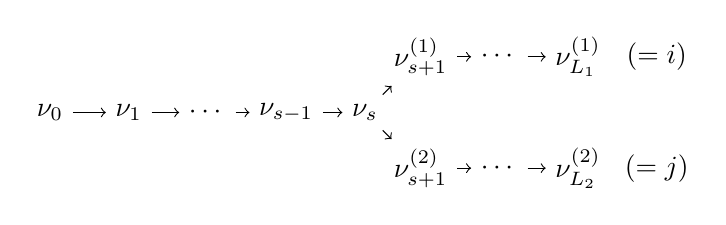
\begin{tikzpicture}
\node (nu0) {$\nu_0$};
\node (nu1) [right of=nu0] {$\nu_1$};
\node (dots0) [right of=nu1] {$\cdots$};
\node (nus1) [right of=dots0] {$\nu_{s-1}$};
\node (nus) [right of=nus1] {$\nu_s$};
\node (nu11) [above right of=nus] {$\nu^{(1)}_{s+1}$};
\node (dots1) [right of=nu11] {$\cdots$};
\node (nu1L1) [right of=dots1] {$\nu^{(1)}_{L_1}$};
\node (eq1) [right of=nu1L1] {$(= i)$};
\node (nu21) [below right of=nus] {$\nu^{(2)}_{s+1}$};
\node (dots2) [right of=nu21] {$\cdots$};
\node (nu2L2) [right of=dots2] {$\nu^{(2)}_{L_2}$};
\node (eq2) [right of=nu2L2] {$(= j)$};
%
\draw [->] (nu0) -- (nu1);
\draw [->] (nu1) -- (dots0);
\draw [->] (dots0) -- (nus1);
\draw [->] (nus1) -- (nus);
\draw [->] (nus) -- (nu11);
\draw [->] (nu11) -- (dots1);
\draw [->] (dots1) -- (nu1L1);
\draw [->] (nus) -- (nu21);
\draw [->] (nu21) -- (dots2);
\draw [->] (dots2) -- (nu2L2);
\end{tikzpicture}
\end{center}

With this notation, we can integrate over all the random vectors $\theta_{d,\nu}$ and write
{
% TODO: resize / reformat?
\newcommand{\prefix}{\int_{\tilde \theta_d \in \Theta_d} \tallbracketl{[}{5ex}}
\begin{align*}
%\MoveEqLeft
R_{i,j}
={}&P(\pi_{d,1} = i, \pi_{d,2} = j)
\\
={}&
\prefix
  P\left(\pi_{d,1}=i \,|\, \{ \theta_{d,\nu} = \tilde \theta_{d,\nu} \}_{\nu \in \nonTerm(T)}\right)
\\ &\phantom{\prefix}
  \cdot P\left(\pi_{d,2}=j \,|\, \{ \theta_{d,\nu} = \tilde \theta_{d,\nu} \}_{\nu \in \nonTerm(T)}\right)
  \left(
    \prod_{\nu \in \nonTerm(T)} P\left(\theta_{d,\nu} = \tilde \theta_{d,\nu}\right)
  \right)
  \tallbracketr{]}{5ex}
\\
={}&
\prefix
  \left(
    \prod_{k=0}^{s-1} \tilde \theta_{d,\nu_k,\nu_{k+1}}
  \right)
  \tilde \theta_{d,\nu_s,\nu^{(1)}_1}
  \left(
    \prod_{k=s+1}^{L_1-1} \tilde \theta_{d,\nu^{(1)}_{k},\nu^{(1)}_{k+1}}
  \right)
\\ &\phantom{\prefix}
  \cdot
  \left(
    \prod_{k=0}^{s-1} \tilde \theta_{d,\nu_k,\nu_{k+1}}
  \right)
  \tilde \theta_{d,\nu_s,\nu^{(2)}_1}
  \left(
    \prod_{k=s+1}^{L_2-1} \tilde \theta_{d,\nu^{(2)}_{k},\nu^{(2)}_{k+1}}
  \right)
  \left(
    \prod_{\nu \in \nonTerm(T)}
    \frac{1}{B(\vec\alpha_\nu)}
    \prod_{\nu' \in \text{ch}(\nu)}
    \tilde \theta_{d,\nu,\nu'}^{\alpha_{\nu,\nu'}-1}
  \right)
  \tallbracketr{]}{5ex}
\end{align*}
}

Next, we have two cases, depending on whether or not $i$ and $j$ are distinct.
If $i \neq j$, then
\begin{align}
%\MoveEqLeft
R_{i,j}
={}&P(\pi_{d,1} = i, \pi_{d,2} = j)
\nonumber
\\
={}&
\left(
  \prod_{k=0}^{s-1}
  \frac{B(\vec\alpha_{\nu_k} + 2 \vec e_{\nu_{k+1}})}
       {B(\vec\alpha_{\nu_k})}
\right)
\left(
  \frac{B(\vec\alpha_{\nu_s} + \vec e_{\nu^{(1)}_{1}} + \vec e_{\nu^{(2)}_{1}})}
       {B(\vec\alpha_{\nu_s})}
\right)
\nonumber
\\ & \cdot
\left(
  \prod_{k=s+1}^{L_1-1}
  \frac{B(\vec\alpha_{\nu^{(1)}_{k}} + \vec e_{\nu^{(1)}_{k+1}})}
       {B(\vec\alpha_{\nu^{(1)}_{k}})}
\right)
\left(
  \prod_{k=s+1}^{L_2-1}
  \frac{B(\vec\alpha_{\nu^{(2)}_{k}} + \vec e_{\nu^{(2)}_{k+1}})}
       {B(\vec\alpha_{\nu^{(2)}_{k}})}
\right)
\nonumber
\\
={}&
\left(
  \prod_{k=0}^{s-1}
  \frac{(1 + \alpha_{\nu_k,\nu_{k+1}}) (\alpha_{\nu_k,\nu_{k+1}})}
       {(1 + \sum_{\nu'} \alpha_{\nu_k,\nu'}) (\sum_{\nu'} \alpha_{\nu_k,\nu'})}
\right)
\left(
  \frac{(\alpha_{\nu_s,\nu^{(1)}_{1}}) (\alpha_{\nu_s,\nu^{(2)}_{1}})}
       {(1 + \sum_{\nu'} \alpha_{\nu_s,\nu'}) (\sum_{\nu'} \alpha_{\nu_s,\nu'})}
\right)
\nonumber
\\ & \cdot
\left(
  \prod_{k=s+1}^{L_1-1}
  \frac{\alpha_{\nu^{(1)}_{k}, \nu^{(1)}_{k+1}}}
       {\sum_{\nu'} \alpha_{\nu^{(1)}_{k}, \nu'}}
\right)
\left(
  \prod_{k=s+1}^{L_2-1}
  \frac{\alpha_{\nu^{(2)}_{k}, \nu^{(2)}_{k+1}}}
       {\sum_{\nu'} \alpha_{\nu^{(2)}_{k}, \nu'}}
\right)
\label{eqn:cooccurDistinct}
\end{align}

On the other hand, if $i = j$, there are no nodes beyond the split point $\nu_s$, which means $L_1 = L_2 = s$.
Therefore,
\begin{align}
R_{i,i}
&= P(\pi_{d,1} = i, \pi_{d,2} = i)
\nonumber
\\
&=
  \prod_{k=0}^{s-1}
  \frac{B(\vec\alpha_{\nu_k} + 2 \vec e_{\nu_{k+1}})}
       {B(\vec\alpha_{\nu_k})}
\nonumber
\\
&=
\prod_{k=0}^{s-1}
\frac{(1 + \alpha_{\nu_k,\nu_{k+1}}) (\alpha_{\nu_k,\nu_{k+1}})}
     {(1 + \sum_{\nu'} \alpha_{\nu_k,\nu'}) (\sum_{\nu'} \alpha_{\nu_k,\nu'})}
\label{eqn:cooccurSame}
\end{align}

Next, we'll derive a closed-form expression for the entries of the co-occurrence ratio matrix $\Rbar$:
\begin{align*}
\Rbar_{i,j}
&=
\frac{R_{i,j}}{ \bigl( \sum_{j'} R_{i,j'} \bigr) \bigl( \sum_{i'} R_{i',j} \bigr) }
\\
&=
\frac{P(\pi_{d,1} = i, \pi_{d,2} = j)}
     {P(\pi_{d,1} = i) \, P(\pi_{d,2} = j)}
\end{align*}

When we combine the above results, many factors cancel, yielding
\begin{align}
\Rbar_{i,j}
&=
\begin{cases}
\displaystyle
\prod_{k=0}^{s-1}
  \frac{ \left( 1 + \alpha_{\nu_k,\nu_{k+1}} \right) \left( \sum_{\nu'} \alpha_{\nu_k, \nu'} \right) }
       { \left( \alpha_{\nu_k,\nu_{k+1}} \right) \left( 1 + \sum_{\nu'} \alpha_{\nu_k, \nu'} \right) }
&
\text{if } i = j,
\\[4ex]
\displaystyle
\left(
  \prod_{k=0}^{s-1}
    \frac{ \left( 1 + \alpha_{\nu_k,\nu_{k+1}} \right) \left( \sum_{\nu'} \alpha_{\nu_k, \nu'} \right) }
         { \left( \alpha_{\nu_k,\nu_{k+1}} \right) \left( 1 + \sum_{\nu'} \alpha_{\nu_k, \nu'} \right) }
\right)
\left(
  \frac{\sum_{\nu'} \alpha_{\nu_s, \nu'}}
       {1 + \sum_{\nu'} \alpha_{\nu_s, \nu'}}
\right)
&
\text{if } i \neq j,
\end{cases}
\label{eqn:closedFormRbar}
\end{align}

In particular, note that $\Rbar_{i,j}$ can be viewed as a function of the least common ancestor of $i$ and $j$, which we are denoting $\nu_s$.

\subsection{Properties of the Co-occurrence Ratio Matrix}

\begin{defn}[Limited-Sparsity Property]
Suppose a TreePAM model has a Dirichlet parameter vector $\alpha_\nu$ specified for each internal node $\nu$.
We say this model satisfies the \emph{limited-sparsity property} if, for each edge between internal nodes $i \to j$, we have $\sum_k \alpha_{j,k} > \alpha_{i,j}$.
In other words, the sparsity of the Dirichlet distribution associated with each non-root internal node is limited by the Dirichlet parameter corresponding to its parent.
\end{defn}

\begin{claim}
Suppose we have a TreePAM model in which the Dirichlet parameters satisfy the limited-sparsity property.
For any leaf node $i$, the maximum value of $\Rbar_{i,j}$ for $j \neq i$ is attained when $j$ corresponds to either a sibling of $i$ or a descendant of a sibling of $i$.
\label{claim:RbarMatrixProperty}
\end{claim}

We prove this claim using the following lemmas.

\begin{lemma}
If $a$, $b$, and $c$ are three distinct leaf nodes, then $\text{LCA}(a,b) = \text{LCA}(a,c)$ implies $\Rbar_{a,b} = \Rbar_{a,c}$.
\label{lemma:equalLCA}
\end{lemma}

\begin{proof}
This lemma follows from the fact that the expression for $\Rbar_{i,j}$ derived in equation~\eqref{eqn:closedFormRbar} does not depend on any nodes except for those on the path from the root to $\text{LCA}(i,j)$.
\end{proof}

\begin{lemma}
Suppose the premises of Claim~\ref{claim:RbarMatrixProperty} hold, and suppose we have three distinct leaf nodes $a$, $b$, and $c$, where $\text{LCA}(a,b)$ is a strict descendant of $\text{LCA}(a,c)$.
Then $\Rbar_{a,b} > \Rbar_{a,c}$.
\label{lemma:greaterLCA}
\end{lemma}

\begin{proof}
Let $\lambda = \text{LCA}(a,b)$ and let $\mu = \text{LCA}(a,c)$ such that $\lambda$ is a strict descendant of $\mu$.
Thus, the path from the root to $\lambda$ includes $\mu$.
Let the path from the root to $\lambda$ be denoted by
\begin{align*}
\nu_0 \to \nu_1 \to \cdots \to \nu_{s_1} \to \cdots \to \nu_{s_2},
\end{align*}
where $\nu_{s_1} = \mu$ and $\nu_{s_2} = \lambda$ for $s_1 < s_2$.

Using equation~\eqref{eqn:closedFormRbar} and the fact that $a \neq b$ and $a \neq c$, we can compute
\begin{align}
\frac{\Rbar_{a,b}}{\Rbar_{a,c}}
&=
\prod_{k=s_1+1}^{s_2}
\frac
  { \left( 1 + \alpha_{\nu_{k-1}, \nu_k} \right) \left( \sum_{\nu'} \alpha_{\nu_k, \nu'} \right) }
  { \left( \alpha_{\nu_{k-1}, \nu_k} \right) \left( 1 + \sum_{\nu'} \alpha_{\nu_k, \nu'} \right) }
\\
&=
\prod_{k=s_1+1}^{s_2}
\frac
  { \sum_{\nu'} \alpha_{\nu_k, \nu'} + \alpha_{\nu_{k-1}, \nu_k} \sum_{\nu'} \alpha_{\nu_k, \nu'} }
  { \alpha_{\nu_{k-1}, \nu_k} + \alpha_{\nu_{k-1}, \nu_k} \sum_{\nu'} \alpha_{\nu_k, \nu'} }
\end{align}
%
Since we assumed that our model satisfies the limited-sparsity property, we know that $\sum_{\nu'} \alpha_{\nu_k, \nu'} > \alpha_{\nu_{k-1}, \nu_k}$ for all $k$ such that $s_1 < k \leq s_2$; therefore, each factor in the above product is greater than $1$.
Furthermore, since $s_1 < s_2$, we know that the above product contains at least one factor.
Thus, we can conclude $\Rbar_{a,b} > \Rbar_{a,c}$.
\end{proof}

\begin{proof}[Proof of Claim~\ref{claim:RbarMatrixProperty}]
First, suppose $i$ is a leaf node, and let $S$ be the set of all leaves that are either siblings of $i$ or descended from a sibling of $i$.
If $i$ is a leaf with no parent, then $i$ must be the only node in the tree, and Claim~\ref{claim:RbarMatrixProperty} is vacuously true.
Thus, assume $i$ has a parent.

For any $j_1, j_2 \in S$, we know that $\text{LCA}(i, j_1) = \text{LCA}(i, j_2) = \text{parent}(i)$.
Therefore, we have $\Rbar_{i,j_1} = \Rbar_{i,j_2}$ by Lemma~\ref{lemma:equalLCA}.

Next, suppose $j$ is any node in $S$ and $k$ is any node outside of $S$ that is distinct from $i$.
Then, we know that $\text{LCA}(i,j) = \text{parent}(i)$, which must be a strict descendant of $\text{LCA}(i,k)$.
This is because our assumptions imply that $k$ must not be a descendant of $\text{parent}(i)$.
Therefore, $\Rbar_{i,j} > \Rbar_{i,k}$ using Lemma~\ref{lemma:greaterLCA}.
\end{proof}

\begin{claim}
Suppose we have a dataset generated by a TreePAM model based on a tree $T$.
Let $\phi$ be a lower bound on the minimum non-zero within-row difference in the true $\Rbar$ matrix (ignoring entries along the diagonal) corresponding to this model.
That is,
\begin{align*}
\phi \leq \min |\Rbar_{a,b} - \Rbar_{a,c}|,
\end{align*}
where the above minimum is taken with respect to all triplets of leaves $a, b, c \in T$ such that $a \neq b$, $a \neq c$, $b \neq c$, and $\LCA(a,b) \neq \LCA(a,c)$.
Suppose also that we use our dataset to estimate $\Rbar$ with additive error upper-bounded by $\epsilon$, and that $\epsilon \leq \phi/4$.
Then, if we apply our proposed algorithm with a constraint-strength cutoff of $\tau = 2\epsilon \leq \phi/2$, we will pass the following set of constraints to Aho's algorithm:
\begin{align*}
C_T = \{ (\{a,b\},c) \,|\, \LCA(a,b) \text{ is a strict descendant of } \LCA(a,c) \text{ in } T \}
\end{align*}
\end{claim}
\begin{proof}
First, we note that
\begin{gather}
\LCA(a,b) \text{ is a strict descendant of } \LCA(a,c) \label{eqn:strictDesc1} \\
\text{ if and only if } \nonumber \\
\LCA(a,b) \text{ is a strict descendant of } \LCA(b,c). \label{eqn:strictDesc2}
\end{gather}
This is because $a$, $b$, and $c$ are distinct leaves, and since $a$ and $b$ are descendants of $\LCA(a,b)$, we know that
\begin{align*}
\LCA(a,c) &= \LCA(\LCA(a,b),c) = \LCA(a,b,c) \text{ and} \\
\LCA(b,c) &= \LCA(\LCA(a,b),c) = \LCA(a,b,c).
\end{align*}
Using Lemmas~\ref{lemma:equalLCA} and~\ref{lemma:greaterLCA}, the statements \eqref{eqn:strictDesc1} and \eqref{eqn:strictDesc2} are simultaneously both true if and only if
\begin{gather*}
\Rbar_{a,b} > \Rbar_{a,c}
\quad \text{ and } \quad
\Rbar_{a,b} > \Rbar_{b,c}.
\end{gather*}
If two entries of $\Rbar$ within the same row are equal, our noisy estimates for those entries will differ from each other by at most $2\epsilon = \tau$.
If two entries of $\Rbar$ within the same row are distinct, our noisy estimates for those entries will differ from each other by at least $\phi - 2\epsilon \geq 2\epsilon = \tau$.
Therefore,
\begin{gather*}
\Rbar_{a,b} > \Rbar_{a,c}
\quad \text{ and } \quad
\Rbar_{a,b} > \Rbar_{b,c} \\
%
\text{ if and only if } \\
%
\RbarEst_{a,b} > \RbarEst_{a,c} + \tau
\quad \text{ and } \quad
\RbarEst_{a,b} > \RbarEst_{b,c} + \tau.
\end{gather*}
In our proposed algorithm, a triplet constraint $(\{a,b\},c)$ will be passed to Aho's algorithm if and only if it has strength $> \tau$.
This will occur if and only if $\RbarEst_{a,b} > \RbarEst_{a,c} + \tau$ and $\RbarEst_{a,b} > \RbarEst_{b,c} + \tau$, which completes our proof that $C_T$ is the set of constraints that we will pass to Aho's algorithm.
\end{proof}

{\bf TODO: Pick up here}

\paragraph{Tree recovery}
Let us say that a rooted, directed tree is \emph{admissible} if it has no nodes with exactly one child.
If $T$ is any tree, then $T$ satisfies exactly the set of triplet constraints $C_T$ defined above.
That is, $T$ satisfies every triplet constraint in $C_T$ but does not satisfy any other triplet constraints.
(This fact comes directly from the definition of triplet constraints.)
Furthermore, if $T$ is admissible, then it is the only admissible tree to do so.
({\bf TODO: proof})
Thus, Aho's algorithm will output $T$ when given the set of constraints $C_T$.

%%%%%%%%%%

\paragraph{Bound on minimum spacing for ratio-matrix entries}
Suppose the TreePAM model's parameters $\alpha_{\nu,\nu'}$ are bounded above by $\alphaMax$.
Suppose also that they satisfy the limited-sparsity property with a margin of at least $\deltaMin$; that is, for every edge $i \to j$ between internal nodes,
\begin{align*}
\sum_{\nu'} \alpha_{j,\nu'} > \alpha_{i,j} + \deltaMin.
\end{align*}
Then we can use
\begin{align*}
\phi = \frac{\deltaMin}{(1+\alphaMax)(1+\alphaMax+\deltaMin))}
\end{align*}
as a lower bound for $\min |\Rbar_{a,b} - \Rbar_{a,c}|$.
Consequently, if we can estimate $\Rbar$ with additive error upper-bounded by $\epsilon \leq \phi/4$, and if we set our constraint-strength threshold $\tau = 2\epsilon$, our proposed algorithm will exactly recover the true tree $T$.

{\bf TODO: Proof}

%%%%%%%%%%%%

\paragraph{Restricted hypothesis class}
Setting $\deltaMin$ and $\alphaMax$ effectively corresponds to selecting a restricted hypothesis class of TreePAM models.
Once a hypothesis class has been selected, we can then compute $\phi$, and from that we can determine the maximum error tolerance $\epsilon = \phi/4$ and the constraint-strength cutoff $\tau = \phi/2$.
Let's consider some examples of $\phi$ calculations corresponding to concrete settings for $\deltaMin$ and $\alphaMax$.

Example: if $\deltaMin = 1$ and $\alphaMax = 8$, then we can set $\phi = 1/90$, which means we need to be able to estimate $\Rbar$ with additive noise less than $1/(90 \cdot 4) = 1/360$.
We can use a constraint-strength cutoff of $\tau = 1/(90 \cdot 2) = 1/180$.

Example: if $\deltaMin = 1/100$ and $\alphaMax = 100$, then we can set $\phi \approx 9.8 \times 10^{-7}$, which means we need to be able to estimate $\Rbar$ with additive noise less than $\phi/4 \approx 2.45 \times 10^{-7}$.
We can use a constraint-strength cutoff of $\tau = \phi/2 \approx 4.9 \times 10^{-7}$.

These examples illustrate a key tradeoff: a broader hypothesis class requires us to more accurately estimate the $\Rbar$ matrix.

%%%%%%%%%%%

\paragraph{Necessity of both bounds}
Next, we'll show that both of the bounds $\alphaMax$ and $\deltaMin$ are necessary to prevent $\phi$ from becoming arbitrarily small.
Without one or the other, we can force $\phi$ to be arbitrarily close to zero.

Specifically, consider 4-leaf binary tree where the root has $\vec\alpha = (x,x)$ and the two children below the root each have $\vec\alpha = (y,y)$.
If we number the leaves left-to-right as $1$ through $4$, the minimum nonzero difference in $\Rbar$ occurs between
\begin{align*}
\Rbar_{1,2} &= \frac{4(1+x)y}{(1+2x)(1+2y)} \quad \text{and} \\
\Rbar_{1,3} &= \frac{2x}{1+2x},
\end{align*}
corresponding to the triplet constraint $(\{1,2\},3)$.
Then, if we violate the $\alphaMax$ bound, by letting $x = y$ as $x,y \to \infty$, we see that $|\Rbar_{1,2} - \Rbar_{1,3}| \to 0$.
Similarly, this difference can get arbitrarily close to $0$ if we violate the $\deltaMin$ bound, by holding $x$ fixed and letting $y = (x+t) / 2$ as $t \to 0$.

%%%%%%%%%%

\paragraph{Recovering Dirichlet parameters}
In addition to recovering the tree $T$ associated with an unknown TreePAM model, we also wish to recover the Dirichlet parameters $\alpha_{\nu,\nu'}$ associated with the edges of the tree.
In this section, we derive an algorithm for doing so.

Suppose $i$ and $j$ are distinct leaves in $T$.
Combining equations \eqref{eqn:cooccurDistinct} and \eqref{eqn:cooccurSame}, and reusing the same indexing notation, we have
\begin{align}
\frac{R_{i,j}}{R_{i,i}}
&=
\frac
  { \alpha_{ \nu_s, \nu_{s+1}^{(2)} } }
  { 1 + \alpha_{ \nu_s, \nu_{s+1}^{(1)} } }
\left(
  \prod_{k=s+1}^{L_1-1}
    \frac
      { 1 + \sum_{\nu'} \alpha_{ \nu_k^{(1)}, \nu' } }
      { 1 + \alpha_{ \nu_k^{(1)}, \nu_{k+1}^{(1)} } }
\right)
\left(
  \prod_{k=s+1}^{L_2-1}
    \frac
      { \alpha_{ \nu_k^{(2)}, \nu_{k+1}^{(2)} } }
      { \sum_{\nu'} \alpha_{ \nu_k^{(2)}, \nu' } }
\right)
\label{eqn:extractAlphaRecursive}
\end{align}
When the leaves $i$ and $j$ share the same parent $p$, we know that $L_1 = L_2 = s+1$, and the above formula reduces to
\begin{align}
\frac{R_{i,j}}{R_{i,i}}
&=
\frac
  { \alpha_{ p, j } }
  { 1 + \alpha_{ p, i } }
\label{eqn:extractAlphaBaseCase}
\end{align}
In fact, when two distinct nodes $c_a$ and $c_b$ are siblings that share a parent $p$, we can rewrite equation~\eqref{eqn:extractAlphaRecursive} as
\begin{align}
\frac{R^*_{c_a,c_b}}{R^*_{c_a,c_a}}
&=
\frac
  { \alpha_{ p, c_b } }
  { 1 + \alpha_{ p, c_a } },
\label{eqn:extractAlphaSimple}
\end{align}
where
\begin{align*}
R^*_{c_a,c_b}
&= R_{\leaf(c_a),\leaf(c_b)} \cdot \frac{ f_1(c_a, \ldots, \leaf(c_a)) }{ f_0(c_b, \ldots, \leaf(c_b)) },
\\
f_t(\nu_{1}, \ldots, \nu_L)
&=
  \prod_{k=1}^{L-1}
    \frac
      { t + \alpha_{ \nu_k, \nu_{k+1} } }
      { t + \sum_{\nu'} \alpha_{ \nu_k, \nu' } }.
\end{align*}
% \begin{align*}
% R^*_{c_a,c_b}
% &= \frac{ R_{\leaf(c_a),\leaf(c_b)} }{ f(\leaf(c_a), \leaf(c_b)) },
% \\
% f(i, j)
% &=
% \left(
%   \prod_{k=s+1}^{L_1-1}
%     \frac
%       { 1 + \sum_{\nu'} \alpha_{ \nu_k^{(1)}, \nu' } }
%       { 1 + \alpha_{ \nu_k^{(1)}, \nu_{k+1}^{(1)} } }
% \right)
% \left(
%   \prod_{k=s+1}^{L_2-1}
%     \frac
%       { \alpha_{ \nu_k^{(2)}, \nu_{k+1}^{(2)} } }
%       { \sum_{\nu'} \alpha_{ \nu_k^{(2)}, \nu' } }
% \right).
% % TODO: fix this notation
% \end{align*}
The function $\leaf(x)$ can be any deterministic mapping from node $x$ to a leaf descended from (or equal to) $x$.
For example, $\leaf(x)$ might always return the leftmost leaf descendant of $x$.

These formulas suggest an algorithm for extracting the Dirichlet parameters for a TreePAM model.
Using equation~\eqref{eqn:extractAlphaBaseCase} we can first solve for the Dirichlet parameters at the bottom of the tree (specifically, the outgoing edges from nodes that have only leaf nodes as children).
Then, we can repeatedly substitute these values into equation~\eqref{eqn:extractAlphaSimple} and solve for the Dirichlet parameters at the next highest edges in the tree.

If $p$ is a node with children $c_1, \ldots, c_k$, equation~\eqref{eqn:extractAlphaSimple} can be applied to the parameters $\alpha_{p,c_i}$ to yield a linear system of at least $k$ equations with $k$ unknowns.
This system may be overdetermined; therefore, without loss of generality, we can choose the $k-1$ equations involving neighboring siblings (with $c_a = c_i$ and $c_b = c_{i+1}$), plus one additional equation where $c_a = c_k$ and $c_b = c_1$.
The solution to this system can be found using the following formula:
\begin{align}
\alpha_{p,c_i}
&=
\frac
  { \displaystyle
    \sum_{n=0}^{k-1}
    \left(
      \prod_{m=0}^{n-1} R^*_{w(c_i,m), w(c_i,m)}
    \right)
    \left(
      \prod_{m=n}^{k-1} R^*_{w(c_i,m), w(c_i,m+1)}
    \right)
  }
  {
    \displaystyle
    \prod_{j=1}^k R^*_{c_j,c_j} - \prod_{j=1}^k R^*_{c_j,w(c_j,1)}
  }
\label{eqn:extractAlphaExplicit}
\shortintertext{where}
w(c_i,m)
&=
\begin{cases}
c_{i+m}, & \text{if } i + m \leq k, \\
c_{i+m-k}, & \text{if } i + m > k.
\end{cases}
\nonumber
\end{align}

Note that the parameters at each layer of the tree can be solved for in terms of parameters from lower layers in the tree.
We can therefore extract all of the Dirichlet parameters $\alpha_{\nu,\nu'}$ by applying equation~\eqref{eqn:extractAlphaExplicit} during a recursive postorder traversal of the tree.

To make this more concrete, consider a $4$-leaf tree with branching structure $(2,2)$, and suppose we are given the $4 \times 4$ matrix $R$, which has rows and columns indexed by the leaves $3$ through $6$.
The parameters extracted from this algorithm are then
\begin{align*}
\alpha_{13}
&= \frac{ R_{33}R_{43} + R_{34}R_{43} }{ R_{33}R_{44} - R_{34}R_{43} }
&
\alpha_{25}
&= \frac{ R_{55}R_{65} + R_{56}R_{65} }{ R_{55}R_{66} - R_{56}R_{65} }
\\
\alpha_{14}
&= \frac{ R_{44}R_{34} + R_{43}R_{34} }{ R_{33}R_{44} - R_{34}R_{43} }
&
\alpha_{26}
&= \frac{ R_{66}R_{56} + R_{65}R_{56} }{ R_{55}R_{66} - R_{56}R_{65} }
\\
\alpha_{01}
&= \frac{ R^*_{11}R^*_{21} + R^*_{12}R^*_{21} }{ R^*_{11}R^*_{22} - R^*_{12}R^*_{21} }
&
\alpha_{02}
&= \frac{ R^*_{22}R^*_{12} + R^*_{21}R^*_{12} }{ R^*_{11}R^*_{22} - R^*_{12}R^*_{21} }
\shortintertext{where}
R^*_{11}
&= R_{33}
&
R^*_{22}
&= R_{55}
\\
R^*_{12}
&= R_{35} \frac{ (1 + \alpha_{13}) (\alpha_{25} + \alpha_{26}) }
               { (1 + \alpha_{13} + \alpha_{14}) (\alpha_{25}) }
&
R^*_{21}
&= R_{53} \frac{ (1 + \alpha_{25}) (\alpha_{13} + \alpha_{14}) }
               { (1 + \alpha_{25} + \alpha_{26}) (\alpha_{13}) }
\end{align*}

\section{Experimental Results on Simulated Data}

{\bf TODO}

%%%%%%%%%%%%%%%%%%%%%%%%%%%%%%%%%%%%%%%%%%%%%%%%%%%%%%%%%%%%%%%%%%%
\clearpage
\appendix
\section{Properties of the Multivariate Beta Function}

The multivariate beta function has the following useful properties:

\begin{itemize}

\item Property 1:
\begin{align*}
\frac{B(\vec x + \vec e_\ell)}{B(\vec x)}
&= \frac{\Gamma(x_\ell + 1) \, \Gamma(\sum_k x_k)}
        {\Gamma(x_\ell) \, \Gamma(1 + \sum_k x_k)}
= \frac{x_\ell}{\sum_k x_k}
\end{align*}

\item Property 2:
\begin{align*}
\frac{B(\vec x + 2\vec e_\ell)}{B(\vec x)}
&= \frac{\Gamma(x_\ell + 2) \, \Gamma(\sum_k x_k)}
        {\Gamma(x_\ell) \, \Gamma(2 + \sum_k x_k)}
= \frac{(1 + x_\ell) x_\ell}{(1 + \sum_k x_k) (\sum_k x_k)}
\end{align*}

\item Property 3:
If $a \neq b$, then
\begin{align*}
\frac{B(\vec x + \vec e_a + \vec e_b)}{B(\vec x)}
&= \frac{\Gamma(x_a + 1) \, \Gamma(x_b + 1) \, \Gamma(\sum_k x_k)}
        {\Gamma(x_a) \, \Gamma(x_b) \, \Gamma(2 + \sum_k x_k)}
= \frac{x_a \, x_b}{(1 + \sum_k x_k) (\sum_k x_k)}
\end{align*}

\end{itemize}

\end{document}
